% !Mode:: "TeX:UTF-8"

%%%%%%% 正文 %%%%%%%

\chapter{绪论}

\section{研究背景}

语音是人与人交流中最为重要的手段之一,也是实现和谐的人机交互的重要方法。语音合成是人机交互中的关键技术,它使得用户可以通过语音从计算机获取信息与反馈,从而使得人与计算机的交互变得更加和谐自然。


语音合成是人机语音交互的主要技术之一,语音合成技术是通过一些机械的、电子的方法产生人造语音的技术,是实现人机语音通信,建立一个有说话能力的口语系统所必需的关键技术,伴随着电子计算机运算和存储能力的迅猛提升,语音合成有了它新的定义——利用电子计算机和一些专业装置模拟人制造语音的技术。语音合成近些年在技术和应用方面都取得了长足的进展,被应用到不同领域\upcite{1}。


按照人类言语功能的不同层次,语音合成可分成三个层次,它们是: 


1、从文字到语音的合成(Text-To-Speech, TTS); 


2、从概念到语音的合成(Concept-To-Speech, CTS);


3、从意向到语音的合成(Intention-To-Speech, ITS); 


现阶段,语音合成的研究还是集中到文字到语音的合成这一阶段,也就是TTS合成系统。


TTS主要以计算机为媒介,将文本、Word 等各种文字形式的信息,利用语音学的韵律规则合成语音信号并向外部设备进行输出的一种语言处理技术。它的目的就是为了使人们能够更加容易,清晰的听明白文本的内容,赋予计算机一个“嘴巴”,使它通过“说”的方式“背诵”给人们听。目前语音合成技术已经成为各国竞相研究的一个主要内容,它广泛的应用在多媒体技术,语音技术,声学技术甚至图像处理技术上。 


语音合成主要分为两种方法,即参数合成法和波形拼接法。较早前语音合成主要是针对人的发音方式,对发声器官参数进行模拟的参数合成法。进入上个世纪 90年代,波形拼接技术已经在英、法、日、德等国家得到了广泛的研制和应用。这种技术较之前的共振峰技术和 LPC 技术在自然度方面已经有了很大的提高,同时利用PSOLA 算法制造的合成器在应用前景上更大,设计结构也既简单又易于实现。


语音合成经过多年的发展,衔接合成是目前主要的高质量语音合成方法。从长远来看,似乎最有前途的是发音语音合成。而基于声管的语音合成是基于发音机理的语音合成方法的重要组成部分。声道在人体内部,不容易被观测到,这给声道研究带来了一定的技术困难。早期,Edholm 等曾用往尸体的鼻腔灌膜的方法来获得鼻腔形状。Fant 和 Ladefoge也曾用这种方法测量发音人的口腔形状,但这种方法是有局限性的。后来随着科技的进步,X 光摄像、核磁成像等技术都被发明出来,于是对声道的测量也就进入了新的研究阶段。


本研究将基于核磁共振数据,完善现有的元音的声管模型,使模型能生成元音、辅音,提高语音合成的清晰度和自然度并考虑声道的细节形态特征对声学特征的影响。

\section{发展现状}

20世纪是计算机技术迅猛发展的时代,数字化是这个时代的主题,它的发展使得电子技术简单化了,语音合成的发展也证实了这一点。无论是激励声源还是滤波器都可以用数字化方法去实现,从整个系统来看,除了模数和数模转换器以外,就不再需要特殊的硬件设备。另外,随着个人计算机的成熟和推广应用,语音合成研究所需的基本条件有了很大的不同,研究场合不再局限于大的、著名的一些实验室,语音合成的研究开始普及化了,使得更多的人有机会研究语音合成。语音合成技术迎来了迅速的发展,我们进入了计算机语音合成的新时代。此外,计算机存储容量不断增大,运算和检索速度不断提高,大规模真人语音的存储、检索和拼接成为可以实施的工程方案,产生了新的语音合成理论,引起了波形拼接合成、隐马尔可夫参数合成技术的兴起,出现了基于统计参数的语音合成方法。


随着语音学的不断发展,文语转换技术(TTS)已经从最初的满足于声音的可懂性及连贯性逐渐演变为追求语音的高自然度的特性。现在的语音自然度的研究虽然已经成为语音学家们越来越关注的话题,但是其自然度所达到的程度仍然不能满足人们的需求,因此,目前在语音合成的自然度方面各生产厂商仍然在不断地创新。可见,语音合成在未来将会有更大的商业市场和机遇。


衔接合成是目前主要的高质量语音合成方法。尽管他已经接近自然演讲的水平了,其他的语音合成方法仍值得推崇。从长远来看,似乎最有前途的是发音语音合成。它不受任何基本的限制,并且超出纯文本-语音合成的应用程序,例如,发音驱动的面部动画和视觉支持第二语言学习和语言障碍的治疗。此外,语音教育和研究可以受益于发音语音合成。


语音合成作为信息处理领域的一个重要分支,涉及到自然语言理解、语音学、信号处理、心理学、声学、多媒体技术等多个领域,是当今世界强国竞相研究的热门技术之一。语音合成技术必将在更广泛的范围内得到推广和应用。而且发音语音合成会有很大的发展和应用空间。


现在,世界各大国家都在集中力量进行语音合成,这一技术要求很高的领域,尽管我们国家现在只是在通信方面对语音合成投入了比较多的研究精力,但是相信在不久的将来,随着国家队语音行业的重视程度不断提高,人们对语音自然度要求也越来越苛刻,我国将会有更多的企业和部门从事语音合成行业的研究。这样我国将会在语音合成的各个方面与国外的先进技术长期处于竞争的局面,并会在这种良性的竞争中有所收获。


\section{本文研究内容和组织结构}

\subsection{研究内容}
发不同性质的声音时,声道的情况是不同的,大致可以将这些情况分为两大类:



(1)发元音的情况:这时声道中的口腔为稳定的某种形状的谐振腔。由声门来的准周期脉冲波激励声道而产生响应。所有的单元音,复元音及复鼻音的元音部分都属于这种情况。

(2)发辅音的情况:此时又可以分为塞音、擦音、鼻音等情况。发塞音时,声道的某部分构成阻碍,使声道完全封闭,由声门来的激励波在此处形成高压湍流,然后突然开放,发出声音。发擦音时,声道的某部分构成为完全封闭的阻碍,使激励在此处形成高速湍流,与该处摩擦而发出声音。而发鼻音时,软腭下垂,鼻腔参加谐振响应。




对于声道的数学模型,有两种观点:一种是将声道看作是由多个不同的截面积的声管串联而成的系统,称为声管模型;另一种是将声道视为一个谐振腔,共振峰就是这个腔体的谐振频率,从这个角度出发来描述声道的模型,即为共振峰模型。本课题采用的是第一种,即声管模型。


本文将基于核磁共振(MRI)数据,采用时域模拟方法,用传输线电路TLM来模拟声道,并加入了噪声源模型。模型中,控制声波生成和传播的声波方程通过应用一定的规则转化为离散变量,并在基于一个更现实的对流体动压变化的分布式考虑及基础上进行改进,同时考虑声道的分支将三个不同稀疏矩阵运用数学方法合并成单一矩阵,以此来完善现有的元音的声管模型,使模型能更准确的生成元音、辅音,并且可以成功避免声伪像。


\subsection{组织结构}
本论文共包含五个章节,具体组织结构如下。


第一章:绪论。主要描述研究背景,发展现状以及本文研究内容和组织结构。


第二章:相关理论基础。主要介绍一些本文需要的相关知识。


第三章:模型构建。主要描述整个声道模型构建的各个部分。 。。。。。


第四章:结果与分析。   。。。。。。


第五章:总结与展望。对论文工作进行总结以及未来工作展望。


\chapter{相关理论基础}

\section{RIFF/WAV}

\subsection{简介}

RIFF全称为子源互换文件格式(ResourcesInterchange FileFormat),RIFF文件是Windows环境下大部分多媒体文件遵循的一种文件结构,RIFF文件所包含的数据类型由该文件的扩展名来标识,能以RIFF文件存储的数据包括:



·音频视频交错格式数据(.AVI)



·波形格式数据(.WAV)



·位图格式数据(.RDI)



·MIDI格式数据(.RMI)



·调色板格式(.PAL)



·多媒体电影(.RMN)



·动画光标(.ANI)



·其他RIFF文件(.BND)


\subsection{CHUNK}

CHUNK 是组成RIFF文件的基本单元,它的结构如下:



structchunk{
  u32id;/*块标志*/
  u32size;/*块大小*/
  u8dat[size];/*块内容*/
};



·id 由四个ASCII字符组成,用以识别块中所包含的数据。如:‘RIFF’,‘LIST’,‘fmt’,‘data’,‘WAV’,‘AVI’等等,由于这种结构最初是由Microsoft和BM为PC机所定义,RIFF文件是按照little-endian字节顺序写入的。


·size(块大小)是存储在data域中数据的长度,id与size域的大小则不包括在该值内。


·dat(块内容)中所包含的数据是以字(WORD)为单位排列的,如果该数据结构长度是奇数,则在最后添加一个空(NULL)字节。



其中有且仅有两种块:‘RIFF’和‘LIST’块可以包含其他块,而其他块仅能含有数据。

\subsection{WAV格式}
WAVE文件作为作为多媒体中使用的波文件格式之一,它是以RIFF格式为标准的。每个WAVE文件的头四个字节便是”RIFF”。Wav文件由文件头和数据体两部分组成。文件头又分为RIFF/WAV文件标识段和声音数据格式说明段。


WAVE文件是由若干个Chunk组成的。按照在文件中出现的位置包括:RIFF WAVE Chunk,Format Chunk,Fact Chunk(可选),Data Chunk。具体如图~\ref{fig:Wav}~所示。

\begin{figure}[htbp]%并排两张图片
\centering
\begin{minipage}[Wav格式包含Chunk示例]{0.5\linewidth}
\centering
  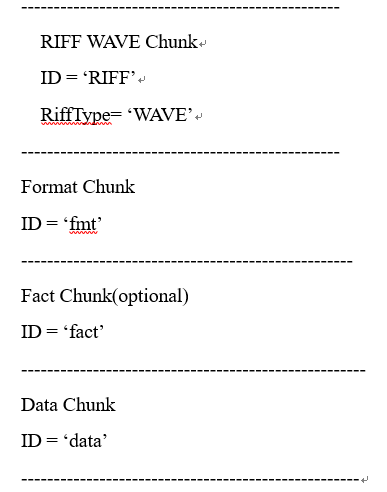
\includegraphics[width=0.5\textwidth,height=5cm]{figures/Wav.png}
\caption{Wav格式包含Chunk示例}\label{fig:Wav}
\end{minipage}%
\begin{minipage}[RIFF WAVE Chunk]{0.5\linewidth}
\centering
 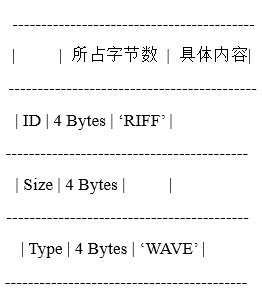
\includegraphics[width=0.5\textwidth,height=5cm]{figures/RIFF.png}
\caption{Wav格式包含Chunk示例}\label{fig:RIFF}
\end{minipage}%  
\end{figure}

图~\ref{fig:Wav}~中除了Fact Chunk 外,其他三个Chunk 是必须的。每个Chunk 有各自的ID,位于Chunk 最开始位置,作为标示,而且均为四个字节。并且紧跟在ID后面的是Chunk大小(去除ID和Size所占的字节数后剩下的其他字节数目),四个字节表示,低字节表示数值低位,高字节表示数值高位。Format Chunk以fmt为标示,一般情况下 Size为16,如果是18的话,最后有附加信息。Fact Chunk是可选字段,一般当wav文件由某些软件转化而成,则包含该Chunk。Data Chunk是真正保存wav数据的地方,以‘data’作为该Chunk的标示;然后是数据的大小;紧接着就是wav数据。


图~\ref{fig:RIFF}~以‘RIFF’为标示,然后紧跟着为size字段,该size是整个wave文件大小减去ID和Size所占用的字节数,即 FileLen-8=Size。然后是Type字段,为‘WAVE’,表示是wav文件。

\section{ 一些相关物理知识}
\subsection{伯努利定理}
在一个流体系统,比如:气流,水流中,流速越快,流体产生的压力就越小。


由不可压,理想流体(不可压缩,不计粘性即粘度为0的流体)沿流管作定常流动时的伯努利定理知,流动速度增加,流体的静压将减少;反之,流动速度减小,流体的静压将增加。但流体的静压和动压之后,称为总压保持不变。动压为$\rho\upsilon^2/2$。

\subsection{雷诺数}

一种可用来表征流体流动情况的无量纲数。


$Re=\rho\upsilon d/\mu$ 
其中 ,$\rho$ \mbox{代表密度};$\upsilon$ \mbox{代表流体速度};$\mu$ \mbox{代表粘性系数};d \mbox{代表特征长度}。

流体力学中表征粘性影响的相似性准则数。


雷诺数较小时,粘滞力对流场的影响大于惯性力,流场中流速的扰动会因粘滞力而衰减,流体流动稳定,为层流。反之,若雷诺数较大时,惯性力对流场的影响大于粘滞力,流体流动较不稳定,流速的微小变化容易发展,增强,形成紊乱。


粘性流体的求解不仅和边界条件有关,而且也和雷诺数有关,若雷诺数很小,则粘性力是主要因素,压力项主要和粘性力项平衡;若雷诺数很大,粘性力项则成为次要因素,压力项主要和惯性项平衡。

\subsection{巴特沃斯滤波器}
巴特沃斯滤波器是一种通频带的频率响应曲线很平坦的信号处理滤波器,也叫最大平坦滤波器。


巴特沃斯滤波器的特点是通频带内的频率响应曲线最大限度平坦,没有起伏,而在阻频带则逐渐下降为零。在振幅的对数对角频率的波特图上,从某一边界角频率开始,振幅随着角频率的增加而逐步减少,趋向负无穷大。


一阶巴特沃斯滤波器的衰减率为每倍频6分贝,每十倍频20分贝。二阶巴特沃斯滤波器的衰减率为每倍频12分贝、三阶巴特沃斯滤波器的衰减率为每倍频18分贝、如此类推。巴特沃斯滤波器的振幅对角频率单调下降,并且也是唯一的无论阶数,振幅对角频率曲线都保持同样的形状的滤波器。只不过滤波器阶数越高,在阻频带振幅衰减速度越快。其他滤波器高阶的振幅对角频率图和低阶数的振幅对角频率有不同的形状。

\subsection{电路相关}
刚度:材料或者结构在受力时抵抗弹性变形的能力。


电导:电阻的倒数,单位:西门子。Grad  


电纳:电抗的倒数,单位:西门子。Srad 


电抗:交流电通过电感或者电容压降时,电压与电流之比,虚数表示,单位:欧姆。

\section{语音学相关知识}
\subsection{声道}

声道是很多动物和及人类都有的一个腔室,从声源(哺乳动物是喉头,鸟类则是鸣管)产生的声音经由此处滤出。在哺乳动物中,声道包括喉腔、咽头、口腔和鼻腔,且在一些非人类的哺乳动物中,有些亦包括气囊。

\subsection{声带}

声带是位于喉部的两瓣左右对称的膜状解剖结构,主要功能是振动以及发声,声带肌肉受迷走神经的控制,可以调整声带的张力,以改变振动频率。


在呼吸时,声带张开,允许肺部与外界的空气交换;在憋气时,声带关闭。在说话、唱歌等动作时,声带通过与空气的相互作用产生振动。声带振动产生的声波是语音中浊音的声源,气流通过气管到了喉部,因为声门附近的气道比较窄,所以气流通过声门的速度加快,根据伯努利定理,气流加快处压力会降低,加上两侧声带粘膜极为松软,于是两片声带就向中央靠近,合拢。紧接着当声门闭合之后,来自肺部的气流无法通过,累积的气体压力降再度将声门推开,如此周而复始便产生振动。

\subsection{声门}

声门是两瓣声带之间的开口。


声门是肺部压出的空气通过声带的出口。发声过程中牵涉到声门的音素称为声门音。声门的大小受到声带的控制,不同的声门大小将导致不同的语音音色,声门闭合时间与气流呼出时间协调一致时,才可能出现自然的噪音。发声时,声门闭合呈现“1”形。闭合状态下 ,呼出气流通过声门,使声带产生振动。


在言语发声中,以声带的振动作为声音源的音称为浊音。

\subsection{发音部位}

发音部位在语音学上指的是辅音发音时,口腔或者咽腔中受到阻碍的位置。

\subsection{发音方法}

发音方法指的是发音时,喉头、口腔、鼻腔节制气流的方式和状态,包括发音时构成阻碍和克服阻碍的方式,气流强弱的情况及声带是否振动等几个方面。

\subsection{协同发音}
协同发音是指发音时在声道中的两个或者偶遇多个不同的部位形成阻碍,这两个阻碍可能同样是完全阻塞(如协同发音的塞音[kp]),或其中一个的阻碍程度比较轻,(如圆唇化的软腭塞音[kw])Catford称前一种情形为‘等同协同发音’,后一种情形为‘非等同协同发音’。

\subsection{辅音}

辅音又叫子音,是气流在口腔或咽头受到阻碍而形成的音。


发音时气流受到发音器官的各种阻碍,声带不一定振动,不够清晰响亮的音素叫辅音,气流从肺里出来时不一定振动声带,通过口腔时受到一定的阻碍,这种主要依靠阻碍发出的音叫做辅音。


辅音是相对元音而言的,而元音是发音时从肺部呼出的气流通过共鸣器作用的口腔,阻力极小并无摩擦声音的语音。辅音是构成音节的重要组成部分,是区别于元音而称呼的。

\begin{itemize}
\item 辅音按照发音部位可以分为:


唇音、双唇音、唇齿音、舌尖音、齿音、卷舌音、齿龈音、齿龈后音、舌面音、硬颚音、唇硬颚音、软腭音、唇软腭音、小舌音、舌根音、咽音、会厌音、喉音。
\item 辅音按照发音方法可以分为:


(1)	鼻音:发音时,气流的口腔通路闭塞,软腭下垂,带音的气流从鼻腔流出。


(2)	塞音(爆音):也叫爆发音或者破裂音,发音时气流完全阻塞,然后突然放开,让气流出来而形成声音。


(3)	擦音:也称“摩擦音”。发音时,气流通路没有完全闭塞,但很狭窄,气流是从窄缝中挤出,因摩擦而成音。


(4)	塞擦音:成阻时气流通路先闭塞,而后转为窄缝状态。发音开始时和塞音一样,收尾时和擦音一样,所以叫塞擦音。


(5)	清浊音:辅音发音时声带的振动模式,发浊辅音时,声带有充分振动。发清辅音时,声带完全不振动。


(6)	边音:发音时,用舌头挡着口腔中央部分的气流通路,使气流从舌头两边流出。


(7)	近音(无摩擦通音)


(8)	闪音(弹音)


(9)	颤音


\item 英语中28个辅音音素


(1)清辅音:[p]、[t]、[k]、[f]、[s]、[$\int$]、[ $\theta$]、[h]、[t$\int$ ]、[tr]、[ts]。


(2)浊辅音:[b]、[g]、[v]、[z]、[$\zeta$]、[e]、[d$\zeta$]、[dr]、[dz]。


(3)鼻音(浊辅音):[m]、[n]、[$\eta$ ]。


(4)舌侧音(浊辅音):[l]、[r]。


(5)半元音(浊辅音)[w]、[j]。

\end{itemize}

\chapter{模型构建}
\section{声学模型}
本课题中采用声道系统的声学模型包括咽管,口腔,以及鼻腔。具体模型如图 ~\ref{fig:Tract}~ 所示。

\begin{figure}[htbp]
\centering
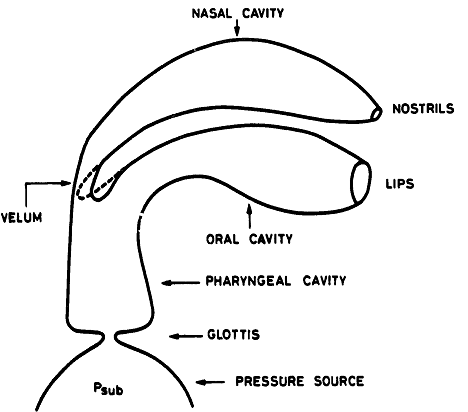
\includegraphics[width=0.5\textwidth]{figures/Tract.png}
\caption{声道系统模型}\label{fig:Tract}
\end{figure}

在该模型中,最内层的咽管通过代表声门孔的狭窄的收缩部分连接到压力源,这个模型中忽略了气管导管(在声门与压力源即肺之间)。当频率低于4KHZ时,声道内的声学波可以被看作是平面波,这是被大家所广泛接受的。


有不同的技术来模拟离散管中声波的传播模型。最常用的技术是基于波数字滤波器,或者基于传输线电路模型的直接数值模拟,或者是基于时域-频域的混合仿真系统模拟声道。每种方法都有其特有的优点和缺点,我们的声学模拟是基于直接数值模拟的传输线电路模型。TLM很容易解释和描述,因为它是直接基于声学和电子系统进行的类比。此外,它没有限制每个管部分的长度。


我们用相邻的不同长度的圆柱管部分来代替声道管。每个管部分由图 ~\ref{fig:Ttype}~  所示的T型网络构成,这样整个管道就可以等价于传输线电路。

\begin{figure}[htbp]
\centering
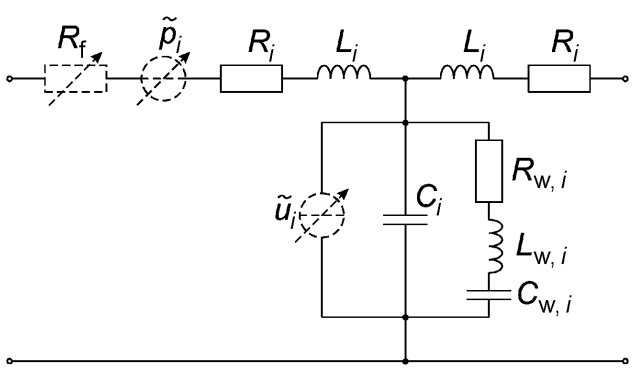
\includegraphics[width=0.5\textwidth]{figures/Ttype.png}
\caption{声道系统模型}\label{fig:Ttype}
\end{figure}

在图3-2中,$L_i$ 是管道i中的空气的惯性,$C_i$ 代表其可压缩性,$R_i$ 代表了整个管壁粘滞摩擦造成的能量损失。$ R_w,_i-L_w,_i-C_w,_i $ 环形电路代表了声道壁的弹性。可选元素 $\tilde{u_i}$,$\tilde{p_i}$ 和 $R_f$ 代表了主要收缩部位的体积速度源,压力源,及动态压降。


在发辅音时声门由面积为0.3$cm^2$,长度为7mm的管来表示。声门到嘴唇之间的面积函数由40个等价的管来表示。

\section{噪声源模型}
几乎所有现有的摩擦音模型都是基于线性source-filter声道模型,并插入一个或多个噪声源来增加声压和体积速度的随机波动,故而,在我们的模型中,也加入了噪声源模型。得到好的噪声源的关键点是适当的参数化噪声源的位置、数量、频谱以及强度。


对于湍流噪声在声管收缩处发生的基本机制有广泛的协议,史蒂文斯总结了至少有三个这样的机制。


1)	气流收缩形成声源,并造成沿着收缩出口向下区域的湍流速度波动。


2)	不规则的几何收缩引起收缩内的随机速度波动。


3)	沿着法线的快速气流撞击在障碍物或者表面从而在中间媒介上产生的波动势力反过来构成声源。


相对于第一种和第二种机制,第三种机制是在产生声压方面最有效的机制[2]。
此外,第三种机制的效率依赖于障碍物的方向以及障碍物和声源之间的距离。气流撞击在法线方向的障碍上会比在较小角度(例如小于90度)方向上撞击获得更大的力量。随着与障碍物的距离增大,声波范围扩大,粒子速度和声源强度都会下降[3]。


根据前两种机制,随机速度波动构成流磁单极子源,并且可以建模为TLM中的体积速度源。根据第三种机制,波动的力量可以构成偶极子源,并且可以建模为TLM中的压力源(图~\ref{fig:Ttype}~中的$\tilde{u_i}$ 和 $\tilde{p_i}$表示了他们在TLM中的位置)。借鉴其他文章([4]),我们提出了一个基于上述机制的噪声源模型,定义了收缩流状况和噪声源的参数的定量关系。参数是通过综合分析实验派生的经验(例如,我们试图通过调整参数来匹配真实的摩擦音频谱和合成频谱)。该模型可以概括如下:


在任何时候,我们假设在声管中只有一个声门收缩,在该处,湍流射流出现。这个流源造成的噪声被建模为一个在收缩出口(流动分离点)的体积速度源$\tilde{u}$,以及假定流源击中一个障碍物或者管道表面部分的压力源$\tilde{p}$。该方法对摩擦音合成的适用性也被Narayanan 和Alwan 所证实了。确定声源的最简单的办法是选择横截面积最小的管截面。然而,当超过一个收缩存在于相同的清晰度的声道时,这可能是模棱两可的。例如,摩擦音/$\int$/,有两个收缩,一个在舌尖,一个在牙齿,他们被舌下空腔所分离。在这种情况下,舌头收缩被认定为是发音的来源。收缩有可能是一连串的管形成的一个狭窄的通道。目前,我们在每个声道的两个分离的部分寻找一个潜在的声源:一个是从声门到舌尖的后一部分,一个是从舌尖到嘴唇的前一部分。选择后一部分还是前一部分作为声源取决于横截面积的和收缩长度。当一个收缩尽可能的长和窄的时候会更有可能被选择。


一旦一个收缩被选中,该模型就可以确定磁单极子和偶极子源的位置。磁单极子总是放在收缩的最前部分,即我们假定流动分离的地方。偶极子源总是放在一个代表性的障碍的位置。当流动分离点(FSP)距离牙齿小于4$cm$时,偶极子源是放在牙齿的,因为这是用来发齿槽音和后齿龈音的。相反,对于软腭音的摩擦音,它被放置在FSP下游0.5$cm$的地方。在后一种情况下,我们假设声道墙作为障碍物。当FSP在牙齿处或者牙齿下游的时候,偶极子源放置在嘴唇的地方。


噪声源只是在某些流条件下被激活。当收缩中的雷诺数的平方$Re^2$小于一定的阈值$Re_crit^2 $时,不会有任何的噪声。否则,辐射噪声声压与$Re^2-Re_crit^2$成正比。在我们的模型中,我们用这个基本依赖来确定磁单极子源的振幅$\tilde{u}$ ̃和压力源的振幅$\tilde{p}$。根据经验公式:









由公式

\[E = mc^2\]

\noindent 下面列出了一些应采用直立数学字体的数学常数和数学符号。

\vspace{-0.5em}
\begin{center}
\begin{tabularx}{0.7\textwidth}{XX}
$\mathrm{d}$、 $\mathrm{D}$、 $\mathrm{p}$~———微分算子 & $\mathrm{e}$~———自然对数之底数 \\
$\mathrm{i}$、 $\mathrm{j}$~———虚数单位 & $\piup$———圆周率\\
\end{tabularx}
\end{center}


出现在正文一行之内的公式称为行内公式,例如~$f(x)=\int_{a}^{b}\frac{\sin{x}}{x}\mathrm{d}x$。对于非矩阵和非多行形式的行内公式,一般不会使得行距发生变化,而~Word~等软件却会根据行内公式的竖直距离而自动调节行距,如图~\ref{fig:hangju}~所示。

\begin{figure}[htbp]
\centering
\subfigure[由~\LaTeX~系统生成的行内公式]{\label{fig:subfig:latex}
                \fbox{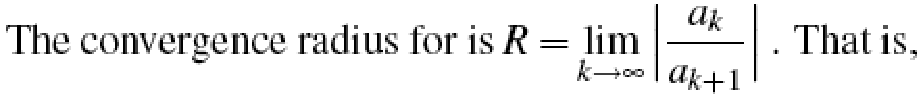
\includegraphics[width=0.55\textwidth]{latex}}}
\subfigure[由~Word软件生成的~.doc~格式行内公式]{\label{fig:subfig:word}
                \fbox{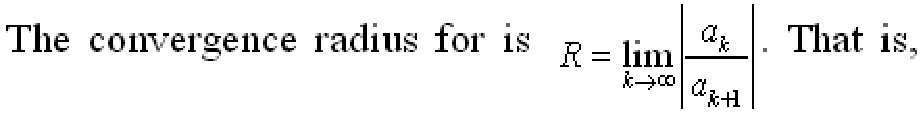
\includegraphics[width=0.55\textwidth]{word}}}
\subfigure[由~Word软件生成的~.pdf~格式行内公式]{\label{fig:subfig:pdf}
                \fbox{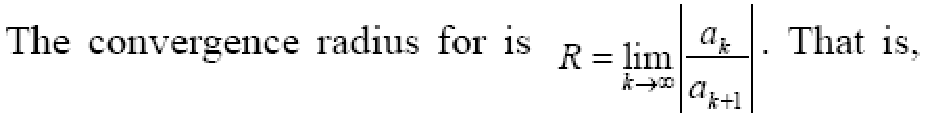
\includegraphics[width=0.55\textwidth]{pdf}}}

\caption{由~\LaTeX~和~Word~生成的~3~种行内公式屏显效果}\label{fig:hangju}
\vspace{-1em}
\end{figure}

\section{代码环境}

很多和计算机专业背景相关的同学都会使用到代码环境,使用~\verb|\verb|~指令或者是~\verb|verbatim|~环境固然是一种选择,但是比不上专门的~lstlisting~环境这么专业。

\begin{lstlisting}
int main(int argc, char ** argv) {
    printf("Hello world!\n");
    return 0;
}
\end{lstlisting}

\noindent\hrule
\vspace{0.1em}\noindent\hrule

\vspace{1em}

\section{普通表格的绘制方法}

表格应具有三线表格式,因此需要调用~booktabs~宏包,其标准格式如表 \ref{tab:table1} 所示。
\begin{table}[htbp]
\caption{符合本科生毕业论文绘图规范的表格}\label{tab:table1}
\vspace{0.5em}\centering\wuhao
\begin{tabular}{ccccc}
\toprule[1.5pt]
$D$(in) & $P_u$(lbs) & $u_u$(in) & $\beta$ & $G_f$(psi.in)\\
\midrule[1pt]
 5 & 269.8 & 0.000674 & 1.79 & 0.04089\\
10 & 421.0 & 0.001035 & 3.59 & 0.04089\\
20 & 640.2 & 0.001565 & 7.18 & 0.04089\\
 5 & 269.8 & 0.000674 & 1.79 & 0.04089\\
10 & 421.0 & 0.001035 & 3.59 & 0.04089\\
20 & 640.2 & 0.001565 & 7.18 & 0.04089\\
 5 & 269.8 & 0.000674 & 1.79 & 0.04089\\
10 & 421.0 & 0.001035 & 3.59 & 0.04089\\
20 & 640.2 & 0.001565 & 7.18 & 0.04089\\
 5 & 269.8 & 0.000674 & 1.79 & 0.04089\\
10 & 421.0 & 0.001035 & 3.59 & 0.04089\\
20 & 640.2 & 0.001565 & 7.18 & 0.04089\\
\bottomrule[1.5pt]
\end{tabular}
\vspace{\baselineskip}
\end{table}

就是这样。

%%%%%%% 结论 %%%%%%%

\addcontentsline{toc}{chapter}{结\quad 论} %添加到目录中

\chapter*{结\quad 论}

得出结论,楼主傻逼。